\subsubsection{XL6009}

El regulador conmutado elevador (o Boost converter en inglés) es un módulo que permite elevar una tensión de entrada más baja a una tensión de salida mayor. Esto se logra gracias a un interruptor (transistor) controlado que conecta una bobina a la alimentación, almacenando mucha energía en forma de campo magnético y redirigiéndola en forma de corriente a través de un diodo al circuito, filtrando a través de un condensador. Una consecuencia es que incrementa la corriente requerida proporcionalmente a la relación de tensión elevada. \cite{xlsemi400KHz604}

En este caso, se utiliza para elevar la tensión de la batería de backup (tensión de $12 V$) a una tensión de $24 V$ para alimentar el sistema, ocupando el lugar del panel cuando este no esté disponible.

\begin{figure}[H]
    \centering
    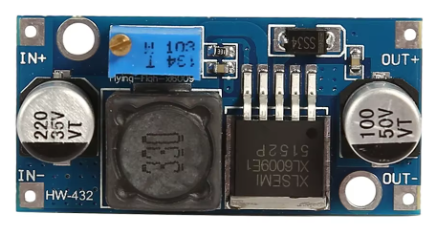
\includegraphics[width=0.5\textwidth]{images/2-hardware/componentes/XL6009.png}
    \caption{Módulo regulador elevador \texttt{XL6009}}
    \label{fig:hardware/modulos/xl6009}
\end{figure}

Con el fin de caracterizar el rendimiento, se han medido las tensiones y corrientes de entrada para dos valores de resistencia, calculando el rendimiento en ambos casos.

\begin{table}[H]
    \centering
    \begin{subtable}[t]{\textwidth}
        \centering
        \begin{tabular}{rrrrr}
            \toprule
            \multicolumn{1}{c}{Carga} & \multicolumn{1}{c}{$V_{in}$} & \multicolumn{1}{c}{$I_{in}$} & \multicolumn{1}{c}{$V_{out}$} & \multicolumn{1}{c}{$I_{out}$}\\ \midrule
            $900\ \Omega$             & $11.87722\ V$                 & $83.476\ mA$                 & $24.9900\ V$                  & $27.415\ mA$                \\
            $450\ \Omega$             & $11.74912\ V$                 & $148.190\ mA$                & $24.9781\ V$                  & $54.196\ mA$                \\ \bottomrule
        \end{tabular}
        \caption{Medidas tomadas en laboratorio}
    \end{subtable}
    \\[0.5cm]
    \begin{subtable}[t]{\textwidth}
        \centering
        \begin{tabular}{rrrr}
            \toprule
            \multicolumn{1}{c}{Carga} & \multicolumn{1}{l}{$P_{in} = V_{in}\cdot I_{in}$} & \multicolumn{1}{l}{$P_{out} = V_{out}\cdot I_{out}$} & \multicolumn{1}{l}{$\eta = 100\%\cdot\frac{P_{out}}{P_{in}}$} \\ \midrule
            $900\ \Omega$             & $0.991\ W$                                     & $0.685\ W$                                        & $69.1\%$                                                    \\
            $100\ \Omega$             & $1.741\ W$                                    & $1.353\ W$                                       & $77.75\%$                                                    \\ \bottomrule
        \end{tabular}
        \caption{Cálculos de rendimiento realizados}
    \end{subtable}
    \caption{Caracterización del rendimiento del LM2596}
    \label{tab:rendimiento_elevador}
\end{table}

Como se puede ver, el rendimiento incrementa con la corriente, como es natural en los reguladores conmutados, por lo que en nuestra aplicación se pueden esperar rendimientos incluso mejores.